\RequirePackage{luatex85}
\documentclass[tikz, border=10pt]{standalone}

\usepackage[compat=1.1.0]{tikz-feynman}

\begin{document}

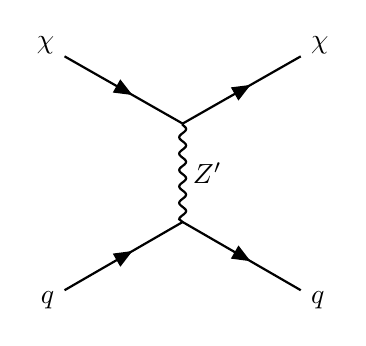
\begin{tikzpicture}[thick]
 \begin{feynman}
  \vertex (origin);
  \vertex [below=1.25cm of origin] (Zprime);
  \vertex [above left=0.75cm and 1.5cm of origin] (chi1) {\(\chi\)};
  \vertex [above right=0.75cm and 1.5cm of origin] (chi2) {\(\chi\)};
  \vertex [below left=0.75cm and 1.5cm of Zprime] (q1) {\(q\)};
  \vertex [below right=0.75cm and 1.5cm of Zprime] (q2) {\(q\)};
  \diagram* {
  (origin) -- [boson, edge label={\(Z^{\prime}\)}] (Zprime),
  (chi1) -- [fermion] (origin) -- [fermion] (chi2),
  (q1) -- [fermion] (Zprime) -- [fermion] (q2)
  };
 \end{feynman}
\end{tikzpicture}
\end{document}
